\documentclass{article}



\usepackage[numbers]{natbib}
\usepackage[french]{babel}
\usepackage[utf8]{inputenc}
\usepackage{amsmath,amssymb}
\usepackage{hyperref}
\usepackage{graphicx}
\usepackage{graphicx}  
\usepackage{float}     
\usepackage{caption}   
\usepackage{subcaption} 

\hypersetup{
    colorlinks=true,
    linkcolor=black,
    pdfborder={0 0 0} 
}

\newcommand{\nbR}{\ensuremath{\mathrm{I\!R}}} % IR

%%%%%%%%%%%%%%%% Lengths %%%%%%%%%%%%%%%%
\setlength{\textwidth}{15.5cm}
\setlength{\evensidemargin}{0.5cm}
\setlength{\oddsidemargin}{0.5cm}

%%%%%%%%%%%%%%%% Variables %%%%%%%%%%%%%%%%
\def\projet{4}
\def\titre{Equations non linéiares et Méthode de Newton-Raphson}
\def\groupe{3}
\def\equipe{4}
\def\responsible{Mohamed Belhassen Charbaji}
\def\secretary{Eve Turchet}
\def\others{Soufiane Sbai,\\ Pierre-Louis Shrestha--Salié}

\begin{document}

%%%%%%%%%%%%%%%% Header %%%%%%%%%%%%%%%%
\noindent\begin{minipage}{0.98\textwidth}
  \vskip 0mm
  \noindent
  { \begin{tabular}{p{7.5cm}}
      {\bfseries \sffamily
        Projet \projet} \\
      {\itshape \titre}
    \end{tabular}}
  \hfill
  \fbox{\begin{tabular}{l}
      {~\hfill \bfseries \sffamily Groupe \groupe\ - Equipe \equipe
        \hfill~} \\[2mm]
      Responsable : \responsible \\
      Secrétaire : \secretary \\
      Codeurs : \others
    \end{tabular}}
  \vskip 4mm ~

  ~~~\parbox{0.95\textwidth}{\small \textit{Résumé~:} \sffamily Ce projet s'intéresse aux algorithmes de recherche de racines d'un système d'équations non linéaires. Nous allons ici considérer la méthode de résolution de Newton-Raphson et son application dans une série de cas concrets.
}
  \vskip 1mm ~
\end{minipage}

%%%%%%%%%%%%%%%% Main part %%%%%%%%%%%%%%%%
\tableofcontents

\section{Méthode de Newton-Raphson}
%TODO INTRODUCTION POUR LE TRUC
La méthode de Newton-Raphson est une méthode itérative permettant le calcul de racine d'une fonction en utilisant 
une approximation locale de la fonction $f$ par sa tangente en un point donné.
subsection{Définition}
La méthode de Newton-Raphson peut être définie de la manière suivante : \\
%% \begin{algorithm}
%% \caption{Méthode de Newton-Raphson}
%% \KwData{Une fonction $f : \mathbb{R}^n \to \mathbb{R}^m$ \\
%%         Un vecteur initial $U$ \\
%%         La matrice Jacobienne de $f$ notée $H$}
%% \KwResult{Un vecteur $U$ approximant une racine de $f$}
%% \While{non convergence de la solution}{
%%     Calculer $f(U)$ et $H(U)$\;
%%     Soit $V$
%%     Résoudre $H(U) V = -f(U)$ pour $V$\;
%%     Mettre à jour $U \gets U + V$\;
%%     $k \gets k + 1$\;
%% }
%% \Return{$U$}
%% \end{algorithm}
\begin{itemize}
  \item Soit la fonction continue  $f$ : $ \mathbb{R}^n \to \mathbb{R}^m $
  \item Soit $ H $ la jacobienne de $f$.
  \item Soit un vecteur arbitraire de $\mathbb{R}^n$.
\end{itemize}
On cherche le vecteur $V$ qui résout le système non linéaire : $f(U + V) = 0$.\\
Le vecteur $U$ est alors actualisé en utilisant $V$: $U \gets U + V$ \\
La méthode est répétée jusqu'à une convergence de la solution $U$, soit lorsque $||f(U)|| < \epsilon$.



\subsection{Méthode de calcul de $V$}
La définition actuelle de $V$ ne permet pas un calcul numérique de $V$ simple.
Nous allons donc définir une relation entre $H, U$ et $ V$ permettant ce calcul.
En utilisant l'approximation :
\[
f(U + V) \approx f(U) + H(U)\cdot V
\]
Or, par définition $V$ est le vecteur tel que $f(U + V ) = 0$, donc on en déduit : $f(U) + H(U)\cdot V \approx 0 $
Calculer $V$ revient à résoudre le système linéaire :
\[
H(U)\cdot V = -f(U)
\]
Cette résolution peut se calculer numériquement grâce à des librairies Python telles que Numpy \citep{numpy_equalin}.
%Sachant que $f(U + V ) = 0$ et $f(U + V)$ est approximée par $f(U) + H(U)\cdot V$ \\
%On trouve alors que \[
%H(U)\cdot V \approx - f(U)
%\]
%Parler du backtracking


\subsection{Backtracking}
En réécrivant l'équation $H(U)\cdot V = -f(U)$, nous obtenons : 
\[ V = -H(U)^{-1}\cdot f(U) \]
L'inverse de la jacobienne de $f$ n'étant pas définie continue, les valeurs singulières de cette dernière peuvent entraîner des étapes instables et conduire à une divergence de la méthode.\\
Nous pouvons utiliser le principe de "backtracking" afin de garantir une convergence de la solution.\\
En utilisant la condition d'Armijo : $ || f(U+t\cdot V)|| > || f(U) + \alpha \cdot t \cdot ||V||$
\\
\begin{itemize}
  \item $t \in [0,1]$ le pas de réduction 
  \item $\alpha \in [0,1] $ le degré d'erreur induite acceptable
\end{itemize}
Nous pouvons itérer en actualisant la valeur de $t$  d'un facteur $\beta \in [0,1[$ jusqu'à ce que la condition soit fausse.\\ 
La valeur de la prochaine itération de $U$ dans la méthode de Newton-Raphson est alors proportionnelle à $t$  : $U = U + t\cdot V$.

\subsection{Vitesse de convergence}

La méthode de Newton-Raphson est réputée pour sa convergence quadratique, ce qui signifie que l'erreur entre l'approximation actuelle et la solution exacte diminue approximativement au carré à chaque itération, sous hypothèse de régularité de $f$.  

Plus précisément, si $U_k$ est l'approximation à l'itération $k$ et $U^*$ la solution exacte, alors dans les cas favorables, l'erreur $\| U_{k+1} - U^* \|$ satisfait la relation suivante :  
\[
\| U_{k+1} - U^* \| \leq C \| U_k - U^* \|^2
\]
où $C$ est une constante dépendant de la fonction $f$. Cette propriété implique une amélioration exponentielle de la précision au fil des itérations.  

Le graphique \ref{fig:convergence_newton} illustre cette convergence rapide en montrant la décroissance de la norme de l'erreur $\| f(U_k) \|$ au fil des itérations :

\begin{figure}[h]
    \centering
    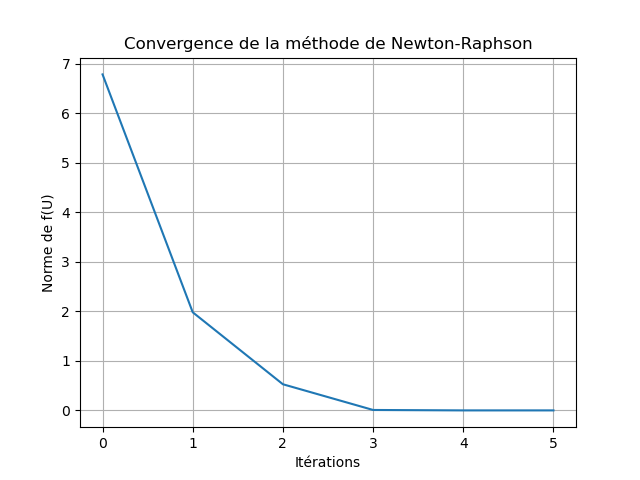
\includegraphics[width=0.8\textwidth]{newton_raphson_convergence.png}
    \caption{Illustration de la convergence quadratique de la méthode de Newton-Raphson}
    \label{fig:convergence_newton}
\end{figure}

\newpage
On constate que, après quelques itérations, l'erreur diminue de manière significative, ce qui confirme la nature quadratique de la convergence et l'efficacité de la méthode dans les cas où elle est applicable.


\section{Méthode de Braistow}
Cette section est une application de la méthode de Newton-Raphson à une fonction spécifique afin de déterminer toutes les racines réelles et complexes d'un polynôme.

\subsection{Explication de l'algorithme}

L'algorithme de Bairstow sert à déterminer toutes les racines d'un polynome P de degré n. Dans un premier temps, cette méthode consiste à calculer tous les facteurs quadratiques $X^{2} + BX + C$ de ce polynome. Dans un second temps, les racines de ces facteurs quadratiques sont calculées.

\bigskip

\indent On considère une fonction vectorielle F(B, C) définie de $\nbR^2$ vers $\nbR^2$ par $F(B, C) = (R, S)$. Les termes B et C sont les coefficients du polynome quadratique $X^{2} + BX + C$. Les termes R et S sont respectivement le coefficient de X et le terme constant du reste de la division de P(X) par $X^{2} + BX + C$.

\bigskip

\indent Trouver les zéros de  cette fonction F revient à déterminer $F(B, C) = (0, 0)$.
Cette équation est vérifiée lorsque que $X^{2} + BX + C$ divise exactement P(X). Les termes B et C sont donc calculés par la méthode de Newton-Raphson.

\bigskip

\indent Chaque zéro (B, C) de F correspond ainsi à un facteur quadratique de P(X), ce qui permet d'extraire deux racines (réelles ou complexes conjuguées) de P(X) sans avoir à manipuler directement des nombres complexes.

Les quatre dérivées partielles de la fonction vectorielle F sont $\frac{\partial R}{\partial B}$, $\frac{\partial R}{\partial C}$, $\frac{\partial S}{\partial B}$ et $\frac{\partial S}{\partial C}$.
\bigskip

\noindent Les dérivées partielles par rapport à C sont obtenues par les équations~\eqref{eq1}.

\begin{equation}
    \frac{\partial R}{\partial C} = -R_1 \hspace{1cm} et \hspace{1cm}
    \frac{\partial S}{\partial C} = -S_1
    \label{eq1}
\end{equation}

\noindent Les dérivées partielles par rapport à B sont elles données par les équations~\eqref{eq2}.

\begin{equation}
    \frac{\partial R}{\partial B} = BR_1 - S_1 \hspace{1cm} et \hspace{1cm}
    \frac{\partial S}{\partial B} = CR_1
    \label{eq2}
\end{equation}

\subsection{Applications de l'algorithme}

L'application de l'algorithme de Bairstow sur différents polynômes a permis d'analyser les
performances de ce dernier.

\begin{figure}[!h]
    \centering
    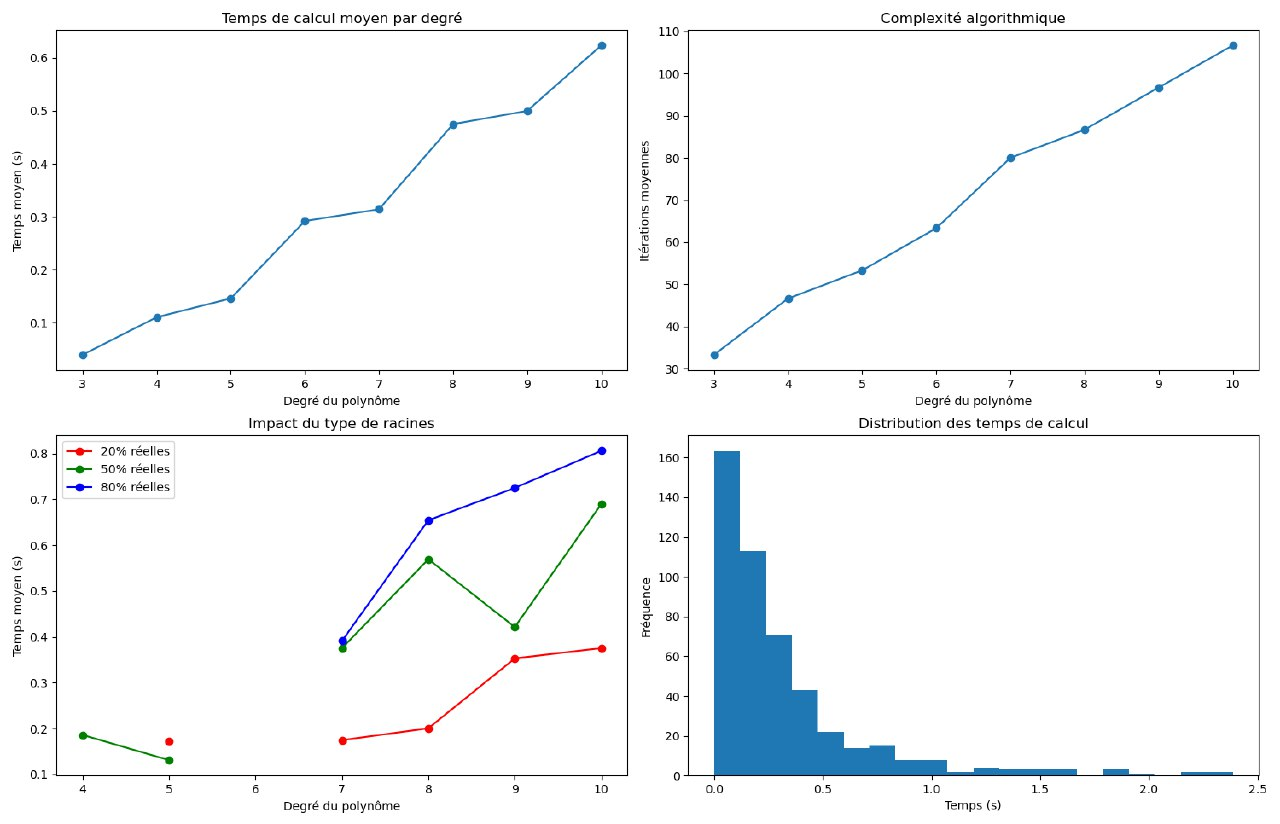
\includegraphics[width=0.90\textwidth]{graphs_bairstow.jpg} 
    \caption{Performances de l'algorithme de Bairstow}
    \label{fig:graph_bairstow} 
\end{figure}

\bigskip

Le graphique en haut à gauche de la figure~\ref{fig:graph_bairstow} indique que plus le degré du polynôme est élevé, plus 
le temps de calcul moyen augmente. Cela suggère que la complexité du calcul croît avec le degré du polynôme.\\

De même, le graphique en haut à droite de la figure~\ref{fig:graph_bairstow} montre une augmentation d'itérations avec le degré du
polynôme. Le temps de calcul est donc directement impacté.

\bigskip

Nous observons également d'après le graphique en bas à gauche de la figure~\ref{fig:graph_bairstow} que le temps de calcul moyen augmente avec le degré du polynôme quelle que soit la proportion
de racines réelles. De plus, l'algorithme prend plus de temps pour les polynômes avec plus de racines réelles.
Cela montre que l'algorithme de Bairstow est plus efficace pour les polynômes ayant principalement des racines
complexes.

\bigskip

La majorité des calculs de l'algorithme de Bairstow sont réalisés en un temps proche de 0 comme le montre
le graphique en bas à droite de la figure~\ref{fig:graph_bairstow}. Cependant, malgré l'efficacité de l'algorithme, il existe 
certains cas pour lesquels le temps de calcul est plus élevé. Cela peut être dû à des polynômes plus complexes
à résoudre.



\section{Points de Lagrange}
Nous allons voir une application de la méthode de Newton-Raphson dans le cadre des points de Lagrange.
\subsection{Définition }
Les points de Lagrange sont des points dans un système à trois corps,où le troisième corps de masse négligeable se trouve à un point d'équilibre.\\
Les forces gravitationnelles et centrifuge s'exerçant sur ce corps se compensent. Permettant à ce corps de rester stable par rapport aux deux autres.\\
Soit : 
\begin{itemize}
  \item $F_c$, la force centrifuge s'appliquant sur le corps
  \item $F_{g1}$, la force gravitationnelle exercée par le premier corps massif
  \item $F_{g2}$, la force gravitationnelle exercée par le deuxième corps massif
\end{itemize}
Les points de Lagrange correspondent donc, dans un référentiel $\nbR^2$, aux points $(x,y) \in \nbR^2$ tels que :
\[
 (F_c + F_{g1} + F_{g2})(x,y) = 0
\]
%TODO s'il reste de la place on peut expliciter la formule des forces 
\subsection{Calcul numérique des points de Lagrange}
A partir des formules décrivant les points de Lagrange \cite{lagrandian_points_formule},  nous pouvons définir les points {L1, L2} et {L3}, dans un référentiel $\nbR^2$ comme les points d'ordonnée nulle et d'abscisse correspondant aux racines réelles des polynômes suivant :\\
\begin{align*}
\textbf{L1:} \quad & x^5 + (\mu - 3)x^4 + (3 - 2\mu)x^3 - \mu x^2 + 2\mu x - \mu = 0 \\
\textbf{L2:} \quad & x^5 + (3 - \mu)x^4 + (3 - 2\mu)x^3 - \mu x^2 - 2\mu x - \mu = 0 \\
\textbf{L3:} \quad & x^5 + (7\mu - 3)x^4 + (3 - 3\mu)x^3 + (9\mu - 8\mu^2 - 3)x^2 \\
                  & \quad + (14\mu^2 - 12\mu + 3)x - 7\mu^2 + 6\mu - 1 = 0
\end{align*}

Avec :
\begin{itemize}
  \item{$\mu$, le ratio de masse des deux corps massifs}
  \item{$x$, la normalisation de la distance entre le point de Lagrange et le premier corps massif}
\end{itemize}
Les racines de ces polynômes peuvent être calculées numériquement en utilisant la méthode de Bairstow.
Les points {L4} et {L5} quant à eux, peuvent être obtenus par construction géométrique.



\section{Conclusion}
Ce projet a permis d'aborder les méthodes numériques de résolution d'équations non linéaires, en insistant
 sur la méthode de Newton-Raphson et ses applications. \\
 Nous avons étudié son implémentation dans des cas concrets tels que l'algorithme de Bairstow pour les racines de polynômes 
 et le calcul des points de Lagrange. \\
 Les résultats montrent l'efficacité de Newton-Raphson pour converger rapidement, tout en 
 soulignant ses limites face à des systèmes complexes ou instables. L'algorithme de Bairstow est 
 également performant, bien que son temps de calcul augmente avec le degré du polynôme. 


\bibliographystyle{plainnat}

\begin{flushleft}
  \bibliography{references}
\end{flushleft}

\end{document}
